\documentclass[aspectratio=169]{beamer}

\usepackage[british]{babel}
\usepackage{lipsum}
\usepackage[T1]{fontenc}
\usepackage[utf8]{inputenc}
\usepackage{lmodern}
\usepackage{microtype}
\usepackage{ragged2e}
\usepackage{multicol}
\usepackage{paralist}
\usepackage{ulem}
\usepackage{blindtext}
%Bibliography
\usepackage[backend=biber, style = authoryear, sorting=nyt]{biblatex}
    \bibliography{references.bib}

\renewbibmacro*{cite}{%
  \iffieldundef{shorthand}
    {\ifthenelse{\ifnameundef{labelname}\OR\iffieldundef{labelyear}}
       {\usebibmacro{cite:label}%
        \setunit{\printdelim{nonameyeardelim}}}
       {\printnames{labelname}%
        \setunit{\printdelim{nameyeardelim}}}%
     \usebibmacro{cite:labeldate+extradate}%
     \setunit{\addcomma\space}%
     \usebibmacro{journal}
     \setunit{\addcomma\space}%
     \usebibmacro{title}}
    {\usebibmacro{cite:shorthand}}}

%Graphikeinbindungen
\usepackage{graphicx}
%\usepackage{sidecap}  
\usepackage{pgfplots}
    \pgfplotsset{compat = 1.15}
\usepackage{tikz}
    \usetikzlibrary{calc,quotes,arrows.meta,automata}
    \usetikzlibrary{overlay-beamer-styles}
\usepackage{tikz-dimline}
\usepackage[compat=1.1.0]{tikz-feynman}
%Farbeinstellungen für Hyperlinks und Pythoncode
\usepackage{xcolor}
    \definecolor{myred}  {HTML}{A3061E}
    \definecolor{myblue} {RGB} {0,63,119}
    \definecolor{myyellow} {cmy} {0,0.263,0.741}
    \definecolor{mygreen} {HTML}{0B6E4F}
    \colorlet{myorange} {myyellow!60!myred}
    \colorlet{myviolett} {myred!50!myblue!80}
%für Python code
\usepackage{listings}
	\lstdefinestyle{python}{
	language         = Python                   ,
	basicstyle       = \ttfamily                ,
	keywordstyle     = \color{myred}            ,
	identifierstyle  = \color{myblue}           ,
	stringstyle      = \color{mygreen}          ,
	commentstyle     = \color{black!50}         ,
	numberstyle      = \color{black!50}\tiny    ,
	numbers          = left                     ,
	belowcaptionskip = \baselineskip            ,
	}
%
\usepackage{caption}
    \captionsetup{%
        font=small,%
        format=plain,%
        labelfont=bf,%
        labelsep=colon,%
        margin=10pt,%
        textfont=sl,%
        singlelinecheck=true%
    }
%Gegen Widowline
\usepackage[defaultlines=2,all]{nowidow}
%Mathe-. und Physikdinge
\usepackage{amssymb, amsmath, amsfonts, amsthm, mathtools, nicefrac, bm, dsfont, upgreek}
\usepackage{mathrsfs}
\usepackage{tensor}
\usepackage{fixmath}
    \usefonttheme[onlymath]{serif}
\usepackage{physics,braket,siunitx}
\usepackage{csquotes}
\usepackage{hyperref}
    \renewcommand{\thefootnote}{\roman{footnote}}
%
\renewcommand{\vec}[1]{\bm{#1}}
\newcommand{\mat}[1]{\vphantom{\uuline{#1}}\smash{\uuline{\mkern-1mu \vphantom{\underline{#1}}#1\mkern-1mu}\mkern2mu}}
\newcommand{\uvec}[1]{\vphantom{\underline{#1}}\smash{\underline{\mkern-1mu #1\mkern-1mu}\mkern2mu}}


\title[Bachelor's Colloquium]{Optimization of the Quantum Espresso Density Functional Theory Code for parallel execution on the PHYSnet-Cluster}
\author{Tjark Sievers}
\date{13th July 2022}
\institute[I. ITP -- AG Computational Condensed Matter Theory]{I. Institute of Theoretical Physics}

\usetheme{CCMT}


\begin{document}

{
\setbeamertemplate{footline}{\empty}
\begin{frame}
	\titlepage
\end{frame}
}
\addtocounter{framenumber}{-1}

\begin{frame}
	\frametitle{Motivation}

	

\end{frame}

\begin{frame}
	\frametitle{Speedup}

	\begin{columns}
		\begin{column}{0.5\textwidth}
			How much faster can a problem be solved with \(N\) processors instead of one?
			
			\begin{equation}
				S \coloneqq \frac{T_1}{T_N}
			\end{equation}

			with serial runtime \(T_1\), runtime on \(N\) cores \(T_N\)

			ideal case: every processor needs the same time
			\begin{align}
				T_N = \frac{T_1}{N}
				\implies S = \frac{T_1}{\frac{T_1}{N}} = N
			\end{align}
				
		\end{column}

		\begin{column}{0.5\textwidth}
			\begin{figure}
				\centering
				\includegraphics[width=0.9\textwidth]{figs/amdahl.pdf}
				%\caption{Speedup modeled by Amdahl's law for different portions of strictly serial workload}
				\label{fig:ideal_speedup}
			\end{figure}
		\end{column}
	\end{columns}
\end{frame}

\begin{frame}
	\frametitle{Amdahl's Law}
	
	\begin{columns}
		\begin{column}{0.5\textwidth}
			In reality: several factors limiting parallelization

			Simple model given by \emph{Amdahl's law}:
			\begin{itemize}
				\item split serial time into a strictly serial part \(s\) and one which can be parallelized perfectly \(p\)
				\item normalize serial time \(T_1 = s + p = 1\)
				\item execution time on \(N\) processors: \(T_N = s + \frac{p}{N}\)
				\item speedup: \(S = \frac{T_1}{T_N} = \frac{1}{s + \frac{p}{N}} = \frac{1}{s + \frac{1 - s}{N}}\)
				\item relevant features: limited by \(\nicefrac{1}{s}\), for smaller \(s\): closer to linear speedup
			\end{itemize}
		\end{column}

		\begin{column}{0.5\textwidth}
			\begin{figure}
				\centering
				\includegraphics[width=0.9\textwidth]{figs/amdahl.pdf}
				%\caption{Speedup modeled by Amdahl's law for different portions of strictly serial workload}
				\label{fig:amdahl}
			\end{figure}
		\end{column}
	\end{columns}
\end{frame}

\begin{frame}
	\frametitle{}

	\begin{columns}
	\begin{column}{0.5\textwidth}
	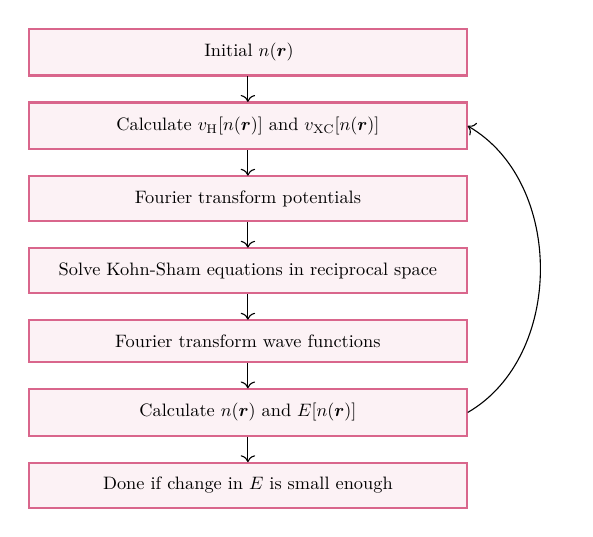
\begin{tikzpicture}[
		scale=0.65,transform shape, squarednode/.style={rectangle, draw=purple!60, fill=purple!5, thick, minimum size=5mm, text centered, text width=8cm,},
		node distance=0.5cm]
		\tikzset{every node/.style={inner sep=8pt}}
		%Nodes
		\node[squarednode]      (init)          {Initial \(n(\vb*{r})\)};
		\node[squarednode]      (step_1)    [below= of init]  {Calculate \(v_{\mathrm{H}} [n(\vb*{r})]\) and \(v_{\mathrm{XC}} [n(\vb*{r})]\)};
		\node[squarednode]      (step_2)    [below= of step_1]      {Fourier transform potentials};
		\node[squarednode]      (step_3)    [below= of step_2]      {Solve Kohn-Sham equations in reciprocal space};
		\node[squarednode]      (step_4)    [below= of step_3]      {Fourier transform wave functions};
		\node[squarednode]      (step_5)    [below= of step_4]      {Calculate \(n(\vb*{r})\) and \(E [n(\vb*{r})]\)};
		\node[squarednode]      (done)      [below= of step_5]      {Done if change in \(E\) is small enough};
		
		%Lines
		\draw[->] (init.south) -- (step_1.north);
		\draw[->] (step_1.south) -- (step_2.north);
		\draw[->] (step_2.south) -- (step_3.north);
		\draw[->] (step_3.south) -- (step_4.north);
		\draw[->] (step_4.south) -- (step_5.north);
		\draw[->] (step_5.east) to [out=30,in=-30] (step_1.east);
		\draw[->] (step_5.south) -- (done.north);
	\end{tikzpicture}
	\end{column}

	\begin{column}{0.5\textwidth}
		
	\end{column}

	\end{columns}
\end{frame}

% Folien für Rückfragen

\begin{frame}
	\frametitle{Factors limiting parallel execution}

	

\end{frame}

\end{document}
